L'objectif commun des deux projets parallèles \eida et \vhs est de
proposer une nouvelle approche de l'étude historique de la circulation
des connaissances scientifiques basée sur de nouvelles méthodes
d'analyse des illustrations. Le développement d'outils numériques pour
l'étude des diagrammes astronomiques -- notamment l'application de
techniques de vision artificielle -- permet d'automatiser une série de
traitements et ainsi de faciliter leur analyse et exploitation. Ces
outils ont pour objectif de réduire les étapes manuelles de fouille et
d'annotation, optimisant ainsi l'efficacité des recherches, et
permettant également de poser un regard neuf sur les objets.

\hypertarget{des-outils-dexploration-et-danalyse-dun-large-corpus}{%
\subsection{Des outils d'exploration et d'analyse d'un large
corpus}\label{des-outils-dexploration-et-danalyse-dun-large-corpus}}

L'ouverture des données met à disposition des chercheur.ses des documents
variés en masse, ce qui a des conséquences profondes sur les
méthodologies de la recherche scientifique.


\subsubsection{EIDA/VHS~: des préoccupations
proches}

\begin{kwote}
"There are tens of thousands of manuscripts and early prints in Latin,
Greek, Arabic/Persian, Sanskrit and Chinese extent today which include
different types of texts, numerical tables and diagrams. Indeed,
astronomers made extensive and refined uses of non-discursive modes of
expression, such as numerical tables and diagrams, in their practice.
The analysis of the precise interactions of the different discursive
(textual) and non-discursive (tables and diagrams) elements that compose
these documents is key to our understanding of a history of astral
sciences that goes beyond the ``surface'' of doctrines and astronomical
models as presented in texts and opens up the potential of the history
of astral sciences for global history".\footcite{husson_eida_2022}.
\end{kwote}       

L'abondance d'archives et de documentation laissées par les astronomes
prémodernes et modernes posent un défi majeur en termes d'exploitation
en raison de la difficulté à mener des études à cette échelle.
Cependant, le traitement par \ia est
prometteur, pour accélérer l'exploration des corpus et interroger les
modalités de circulation des savoirs scientifiques, ainsi que le rôle et
la place de l'image dans la transmission des connaissances. Le but est
de pouvoir donner du sens aux images en évitant au maximum les étape
manuelles d'annotation. Pour ce faire, \eida et \vhs développent des
méthodes d'apprentissage non ou faiblement supervisées permettant
d'effectuer des recherches automatiques à grande échelle dans des corpus
d'envergure. L'utilisation du \dl est centrale pour accomplir
divers traitements analytiques qui accompagnent l'étude des modalités
d'évolution et de transformation des images dans des corpus
scientifiques illustrés.

La collaboration \eida / \vhs a pour but de créer un outil à la fois
polyvalent (une sorte de couteau suisse) et précis, c'est pourquoi il
est nécessaire de différencier et paralléliser les tâches en raison des
finalités spécifiques de chaque projet. Cependant, une base commune
repose sur deux aspects essentiels~: la constitution des corpus
numérisés et l'extraction automatique de leurs illustrations dans une
base de données d'images au format \iiif, dotée d'une interface numérique
de consultation et d'annotation partagée.

\hypertarget{divergences-et-finalites}{%
\subsubsection{Divergences et finalités}\label{divergences-et-finalites}}

Les objectifs de \eida et \vhs sont proches mais des divergences
apparaissent en raison de la nature distincte des corpus, ce qui
entraîne des finalités différentes dans la chaîne de traitement.

Côté \vhs la vision artificielle sert l'analyse d'un large corpus
scientifique illustré du \ma et de la période moderne, ne se
limitant pas aux sciences astronomiques. La méthodologie adoptée
consiste essentiellement à rechercher et identifier (dans un corpus de
manuscrits témoins d'un même travail) les illustrations qui se
correspondent. Cette tâche est ardue pour les ensembles de manuscrits
contenant parfois des centaines d'illustrations, séparés par de
nombreuses copies perdues, s'étalant sur des siècles, et qui ont pu être
complètement réorganisés et fortement modifiés pour s'adapter à de
nouvelles connaissances ou croyances\footcite[``Most research on the
  automatic analysis of manuscripts and particularly their alignment,
  also known as collation, has focused on text. However, illustrations
  are a crucial part of some documents, hinting the copyist values,
  knowledge and beliefs and are thus of major interest to historians.
  One might naively think that these illustrations are much easier to
  align than text and that a specialist can identify them in a matter of
  seconds. This is only true in the simplest of cases, where the order
  of the illustrations is preserved and their content relatively
  similar. In harder cases however, the task becomes daunting and is one
  of the important limiting factor for a large scale analysis.''][p.1]{kaoua_image_2021}.

\begin{kwote}
"{[}N{]}otre approche consiste à concevoir des méthodes basées sur la
vision artificielle pour détecter les similitudes iconographiques
(c'est-à-dire des images qui ont été copiées ou partiellement inspirées
les unes des autres) et textuelles (des images qui décrivent un contenu
textuel similaire mais qui peuvent être visuellement différentes) entre
des illustrations dans de grands corpus. L'un des principaux objectifs
est d'obtenir ces associations automatiquement, en s'appuyant le moins
possible sur les annotations d'experts, qui sont coûteuses et
compliquées à obtenir. Nous faisons l'hypothèse que de telles méthodes
d'analyse permettront d'effectuer beaucoup plus efficacement des
comparaisons et des rapprochements pertinents entre images car elles
fourniront, d'une part, de nouveaux regroupements d'images en fonction
de leur contenu et des textes qu'elles illustrent et, d'autre part, des
distinctions fines entre les différentes modalités de représentation par
l'image."\footcite{noauthor_vision_nodate}.
\end{kwote}       

L'implémentation des méthodes de \dl vise donc essentiellement
la détection automatique de similarités entre les images, ce qui
conduira à la constitution de séries iconographiques~; l'analyse des
associations pouvant être interprétées par les historien.nes.

\begin{kwote}                     
``\vhs associe étroitement deux approches~: d'une part, une approche
historique qui perçoit l'image non pas comme une entité fermée et
isolée, mais comme un vecteur essentiel dans la transmission des
connaissances scientifiques~; d'autre part, le développement de méthodes
automatisées d'analyse des similarités et des contenus dans des corpus
illustrés médiévaux et modernes peu ou pas annotés.''\footcite{noauthor_vision_nodate}
                \end{kwote}       

La phase d'extraction des illustrations garde une place d'importance,
mais la fonctionnalité de vectorisation\footnote{La vectorisation est le
  processus de conversion de données sous forme de listes de structures
  vectorielles, soit une série d'instructions simples, en \xml (au format
  SVG), que l'ordinateur peut traiter très rapidement.} (au cœur des
objectifs d'\eida) se trouve beaucoup moins pertinente, de par le type
d'illustrations présentes dans le corpus \vhs. Plus complexes, elles ne
se prêtent pas -- à l'inverse des diagrammes -- à la décomposition en un
ensemble de formes géométriques élémentaires. En outre la recherche de
similarité constitue une perspective trop ``haut-niveau'' pour les
besoins d'\eida.

\begin{kwote}                     
``However, these approaches typically neither enable fine-grained
control of the reasons images are deemed similar, nor provide a
fine-grained analysis of their content. Moreover, taking into account
data specific or problem specific similarity notions will typically
require the manual annotation of a large scale database, which is
extremely costly and time consuming, limiting practical applications.
Developing alternative solutions to these ``black-box'' deep learning
approaches is thus a critical challenge''\footcite{husson_eida_2022}.
\end{kwote}       

Conformément à cet objectif de produire une analyse détaillée du contenu
des diagrammes, \eida se focalise sur l'algorithme de vectorisation et
extraction des labels, couleurs, et autres caractéristiques sémantiques
spécifiques au diagramme astronomique. La démarche diffère alors de
l'approche plus générique mais plus grossière basée sur les
correspondances\footcite{kaoua_image_2021}, centrale dans \vhs,
qui ne fournit pas le sens \emph{computable} du contenu des images.

\eida adapte des méthodes existantes -- notamment la toute récente
approche ``analysis-by-synthesis''\footnote{L'approche
  ``analysis-by-synthesis'' (analyse par synthèse) en vision par
  ordinateur est une méthode qui consiste à générer des prédictions
  d'objets, puis à comparer ces prédictions avec les données visuelles
  réelles pour vérifier leur précision. Cette approche intègre un cycle
  itératif~: les différences entre les images prédites et les images
  réelles sont ensuite utilisées pour affiner les modèles. En itérant
  alternativement sur la synthèse et l'analyse, cette méthode peut gérer
  une grande gamme de variation dans les données visuelles, elle permet
  ainsi de traiter des problèmes en vision par ordinateur, y compris
  ceux impliquant des données complexes ou ambiguës à l'instar des
  diagrammes astronomiques. Cette approche s'oppose à la ``sketch
  segmentation and labelling'' (\cite{ha_neural_2017}) qui gère mal la
  variabilité et l'ambiguïté des composants. La partie II de ce mémoire
  porte plus spécifiquement sur les méthodes de \cv
  appliquées aux images du projet.} -- pour identifier des primitives
géométriques prédéfinies et gérer les éléments textuels (y compris les
étiquettes de lettres). Les diagrammes sont suffisamment simples pour
être analysés de cette manière, tout en étant suffisamment riches pour
poser des défis significatifs à l'adaptation des méthodes de vision par
ordinateur. Cette méthode permet une description fine et précise du
contenu du diagramme, et surtout retourne un résultat lisible et
compréhensible par la machine, dont l'exploitation se trouve de fait
potentiellement automatisable.

La décomposition des diagrammes astronomiques en composants
significatifs concourt à un double objectif~: leur analyse et leur
édition, en ayant recours au minimum d'annotation humaine.

\begin{kwote}                     
``Central to \eida is the decision to think together issues of diagram
analysis and edition in the context of digital humanities enhanced with
artificial intelligence.''\footcite{husson_eida_2022}
\end{kwote}       

\hypertarget{developpement-dune-interface-commune}{%
\subsection{Développement d'une interface
commune}\label{developpement-dune-interface-commune}}

La gémellité \eida / \vhs tient à leurs objectifs très proches~: la
conception d'instruments d'étude de la circulation des savoirs
scientifiques dans l'histoire au prisme de l'illustration, en exploitant
des méthodes d'analyse par apprentissage profond adaptées à des corpus
anciens. La teneur des outils à concevoir varie, malgré tout il est
nécessaire de développer une application unique pour les deux projets
jumeaux, qui serve de pont entre les utilisateur.rices et les algorithmes de
vision, et permette ainsi le dépôt et le traitement des sources par
l'intermédiaire d'une interface graphique, accessible et utilisable par
les chercheur.ses (dans un premier temps) \footnote{le projet d'une
  interface publique est en préparation}.

Dans ce contexte, le développement en open-source et le partage du code
entre deux projets de recherche offrent plusieurs avantages. Tout
d'abord, cette approche permet de transcender les frontières
disciplinaires, favorisant la transversalité et les discussions
enrichissant les deux projets. La mise en commun des corpus est
notamment bénéfique puisque les sujets de recherche sont connexes.
Ensuite, cette stratégie implique une collaboration entre plusieurs
ingénieur.es, permettant de mutualiser les expertises. Chaque partie peut
ainsi bénéficier des avancées et développements réalisés par l'autre, et
alimenter un savoir-faire collectif. En outre, un problème récurrent
dans le domaine des Humanités Numériques est la dépendance aux logiciels
``maison'' développés en interne et confrontés à des problèmes de
pérennité lorsque les financements s'arrêtent. Le partage des budgets de
recherche et des ressources humaines assure non seulement la durabilité
des outils développés, mais permet également d'aller au-delà des
objectifs initiaux en ouvrant à la continuité des développements.
L'outil n'a pas seulement de meilleures chances d'être maintenu dans le
temps, mais aussi d'évoluer, et le code étant ouvert, l'appui de la
communauté open-source va assurer en partie ces missions. Enfin, éviter
l'écriture de codes redondants s'inscrit dans une stratégie globale de
sobriété, reposant sur l'interopérabilité et l'intégration des outils de
recherche en général, celle-ci gagnant de fait en cohérence et en
efficacité.

Pourtant, la coordination avec une autre équipe ne vient pas sans
contraintes et questionnements. Le développement conjoint implique une
stratégie de programmation modulaire, \emph{a minima} pour répondre aux
besoin d'\eida et \vhs, et qui sera poussée encore plus loin, comme on le
détaillera plus avant\footnote{Voir le \hyperlink{chapitre-3-EDA-image-ia}{chapitre 3}}. Le
développement collaboratif via GitHub constitue une solution pour une
implémentation \emph{à la carte}, garantissant une interaction continue
entre les équipes, tout en offrant la flexibilité de ne pas implémenter
tous les développements effectués dans le cadre du projet parallèle. Les
ingénieur.es des projets \eida et \vhs travaillent sur différentes branches
d'un même dépôt, qui dispose d'une branche pour la mise en production de
l'instance \eida et d'une autre pour la mise en production de
l'instance \vhs. Alors, les développements de l'un ne sont pas
nécessairement mis en production dans le cadre de l'autre, aboutissant à
deux instances indépendantes de la plateforme. L'instance \eida de la plateforme tourne
sur les serveurs de l'observatoire et l'instance \vhs tourne sur le
serveur de la Sorbonne.

La dissociation de l'inférence des modèles de la plateforme
collaborative répond à deux impératifs fondamentaux. D'une part,
l'inférence des modèles requiert une puissance de calcul conséquente,
typiquement fournie par des cartes graphiques \gpu. D'autre part,
l'optimisation des ressources englobe le partage du \emph{hardware}.
L'Observatoire finance donc le \gpu sur lequel tourne l'\api dédiée à
l'exécution des modèles de vision, laquelle est employée par les deux
projets.

Les limites de l'approche collaborative touchent en outre à la
coordination de la temporalité des deux projets. Par exemple,
l'entreprise de refonte du modèle de données pour qu'il s'adapte aux
sources d'\eida, a imposé un ralentissement du côté de \vhs. D'ailleurs,
le défi tenant à la modélisation des données est de taille~: comment
conserver un degré de description suffisant en optant pour la
généralisation des modèles de données~? Nous aborderons cette question
dans la section suivante.

Les difficultés tenant à la coordination des deux équipes sont par
ailleurs apparues dans la mise en œuvre de l'annotation des similarités dans l'optique de \emph{fine-tuner}\footnote{Voir le \hyperlink{fine-tuner-le-modele}{chapitre 5} sur l'entraînement des modèles} le modèle. La
tâche consiste à évaluer à l'aide d'un score les résultats du modèle~:
pour ce faire, cinq catégories ont été définies par les chercheur.ses de
\vhs et le système de notation a été implémenté dans la plateforme avec
les visualisations des résultats. La qualification des similarités
correspond aux catégories 1, 2 et 3. Cette triple catégorisation vise à
différencier les copies exactes (en autorisant des variations minimes
comme celles tenant à un trait à main levée ou au compas) des copies
partielles (notamment dans les imprimées~: une partie d'une \emph{type
form} était souvent réutilisée) de deux images qui représentent un même
contenu intellectuel sans forcément être identiques. La catégorie 4
indique un niveau de similarité non significatif, et la 5 est utilisée
pour n'importe quel type d'association significative entre deux
diagrammes, sans la qualifier. Cette catégorie est spécifique à
l'utilisateur.rice et n'affecte ni l'annotation collective du document ni le
ré-entraînement du modèle. La problématique est alors d'interpréter ces
catégories dans le cadre d'\eida.

La spécificité des diagrammes rend la tâche de définition des catégories
ardue. Déjà, hors du monde de l'imprimé, il est
impossible de trouver de similarité parfaite. En outre, elle ne peut
être recherchée sur des critères autres qu'aspectuels, car des
configurations géométriques semblables peuvent communiquer un contenu
intellectuel très différent compréhensible seulement en contexte et par
un œil expert\footnote{Il convient d'annoter uniquement ce que
  l'algorithme est capable de comprendre, et il n'a accès qu'à l'image.
  Il est impossible de lui apprendre que deux diagrammes, bien que
  visuellement identiques, sont utilisés pour appuyer des arguments
  différents.}.

D'autre part, les diagrammes comportent souvent des labels, et quand un
diagramme franchit des frontières linguistiques, les labels sont
traduits dans un autre alphabet. Donc veut-on que le modèle soit
sensible aux différences de labellisation~? Veut-on que le modèle
considère comme similaire les diagrammes recopiés ayant traversés les
barrières linguistiques~? Si oui il va falloir annoter comme tel les
diagrammes avec des labels divergents, faisant ainsi baisser l'impact de
la labellisation sur le score de similarité. Dans le cas contraire, on
risque d'éloigner des doublons au titre de leur contenu textuel
divergent.

\begin{figure}[H]
          \begin{center}
          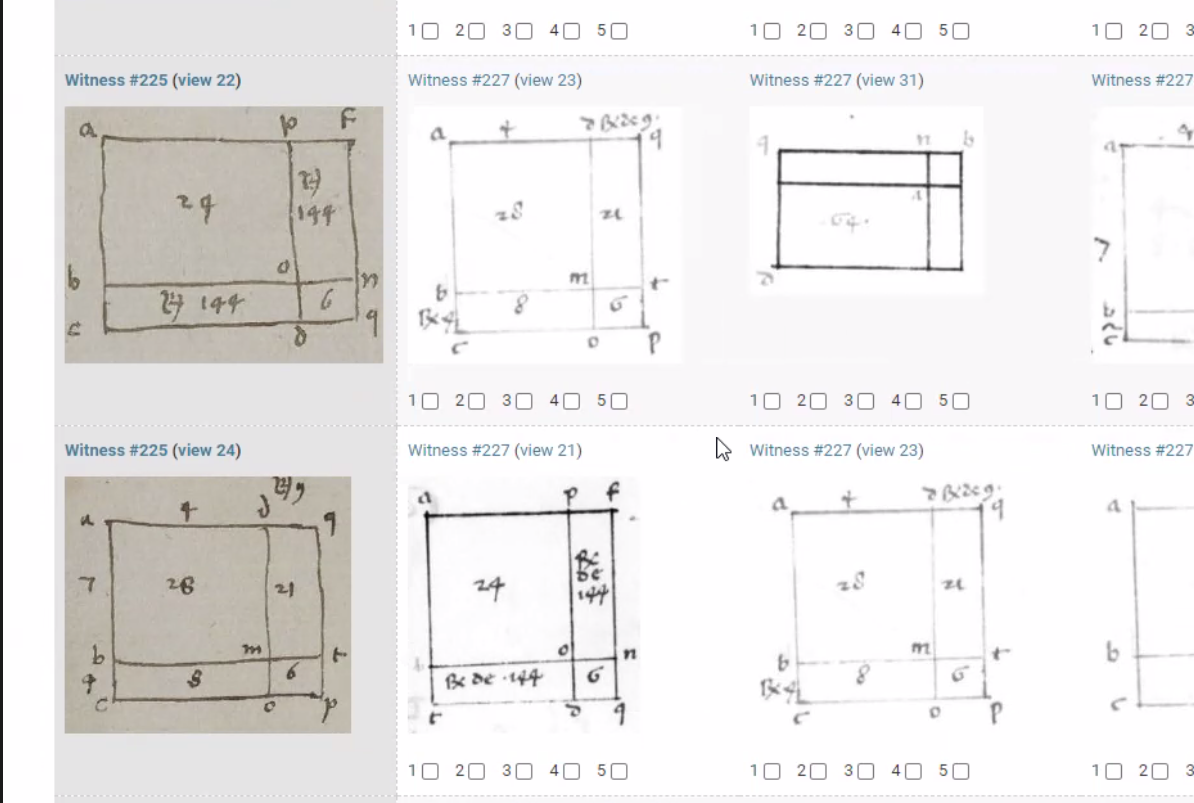
\includegraphics[height=7cm]{figues/label_dissim_exemple.png}
          \end{center}
          \caption{Impact des labels sur la recherche de similarité.}
          \label{fig:simlabel} \end{figure}

Devant ces difficultés il a été décidé d'adopter une annotation binaire
et basée uniquement sur le contenu graphique, partant du principe que
l'assignation d'un score de similarité par le modèle ne vaut pas pour
conclusion historiographique. Il sera toujours plus facile de ne pas
prendre en compte un résultat, et la visée de cet entraînement est
d'aboutir à un modèle assez extensif et généraliste. Il subsiste
cependant des dissensions au sein de l'équipe entre une définition très
stricte de la similarité, quitte à accepter des faux négatifs, et une
définition plus souple (typiquement, sensible aux labels), quitte à
créer des faux positifs. Pour concilier les besoins de tous les
chercheur.ses, il sera recommandé d'annoter selon la définition la plus
rigoureuse d'un point de vue scientifique, cette définition servant de
métadonnée aux chercheur.ses. Les annotations les plus souples seront
utilisées pour l'entraînement du modèle. Cette approche permet de
garantir une précision dans la classification des données tout en
offrant la souplesse nécessaire pour optimiser les performances des
algorithmes d'apprentissage automatique.

Ce cas d'étude est assez caractéristique des enjeux tenant à la
coordination au sein et entre des équipes de recherche dans le cadre du
développement d'un outil commun. D'où le développement des outils
d'annotation dans la plateforme commune assez généralistes pour que leur
usage s'adapte à des besoins différents et complexes\footnote{En
  réalité, les équipes de \vhs sont aussi passées à un classement binaire
  pour prévenir des problèmes de coordination au sein de leurs équipes,
  gardant l'usage des trois autres catégories pour une prochaine étape
  de fine-tuning.}.

\hypertarget{corpus}{%
\subsection{Corpus}\label{corpus}}

Les sources primaires d'\eida couvrent un spectre géographique et
temporel important. Orienté par les objectifs scientifique d'\eida --
arriver à une représentation globale des continuités et divergences qui
se tracent au cœur des pratiques astronomiques à travers l'histoire,
esquisser le voyage des sources à travers le temps et l'espace -- le
refus d'une vision eurocentrée justifie et explique une représentativité
large, servie par la constitution de cinq grands corpus issus de sphères
géographiques et temporelles diverses. Les manuscrits arabo-persans
produits entre le \textsc{viii}\ieme et le \textsc{xiii}\ieme siècle, des manuscrits latins
médiévaux produits majoritairement entre le \textsc{xiii}\ieme et le \textsc{xvi}\ieme siècle, les
manuscrits byzantins, produits entre les \textsc{ix}\ieme et \textsc{xv}\ieme siècles, les
manuscrits sanskrits, à partir du \textsc{xi}\ieme, et enfin les sources chinoises
datant du milieu du \textsc{xvi}\ieme siècle, après l'arrivée des premiers jésuites.
Le support de ces dernières n'est pas nécessairement le manuscrit, elles
prennent souvent la forme d'imprimés par blocs xylographiques dont les
matrices sont réemployées dans plusieurs témoins. Elles présentent donc
une forme hybride, sorte de pré-imprimé, qui posa des questions
complexes pour la modélisation conceptuelle des données.

Plusieurs centaines de manuscrits sont numérisés pour chaque tradition.
Sur ces numérisations, mises à disposition par les institutions
patrimoniales qui conservent ces témoins, seront appliquées les
traitements en prévision de l'analyse par les chercheur.ses, leur
permettant de souligner les motifs qui sous-tendent la diffusion
afro-eurasiens du modèle ptoléméen.

La gémellité avec \vhs impose un effort de modularité pour pouvoir
partager le modèle de données. Le travail de recherche de \vhs est mené
sur quatre corpus relevant, à l'instar de celui d'\eida d'une grande
diversité chronologique et géographique. Ces corpus se distinguent
cependant par une grande diversité thématique~: ils se composent de
manuscrits et d'imprimés concernant les sciences des mathématiques et
les sciences naturelles. Le premier corpus est le \emph{Physiologus},
rédigé vers le \textsc{ii}\ieme siècle à Alexandrie. Ce texte, l'un des plus
populaires du \ma, a contribué à l'émergence de la zoologie
chrétienne médiévale. Il a pour témoins 100 manuscrits grecs, dont treize
sont illustrés et réalisés entre le \textsc{xi}\ieme et le \textsc{xvi}\ieme siècle, contenant
environ 680 images d'animaux, de plantes et de minéraux. Le deuxième
corpus est le \emph{De materia medica} de Dioscoride, composé vers l'an
77 de notre ère. Ce traité pharmacologique destiné aux praticiens a été
largement diffusé et copié. Il est conservé dans 65 manuscrits grecs,
dont 17, réalisés entre le \textsc{vi}\ieme et le \textsc{xvi}\ieme{} siècle, sont illustrés et
contiennent environ 8340 images de plantes, d'animaux et de minéraux.
Les troisième et quatrième corpus se composent des planches de
l'Encyclopédie de Diderot et d'Alembert (1751-1772), les témoins de ce
travail couvrant une longue série de traités, dictionnaires et
encyclopédies au fil desquels les illustrations ont été copiées et
retravaillées. Leur étude se focalise aussi sur leur inclusion
ultérieure dans des encyclopédies telles que l'Encyclopédie méthodique.
Le troisième corpus se concentre sur l'Histoire naturelle (Zoologie),
tandis que le quatrième porte sur les sciences mathématiques\footcite{noauthor_vhs_nodate}.

Le deux corpus jumeaux diffèrent aussi en taille~: celui de \vhs présente plus de 2000 témoins devant 300 pour \eida.

Malgré ces divergences importantes, les données sont issus de spectres
assez larges pour opérer des croisements dont l'exploitation peut
s'avérer fructueuse~: les corpus \vhs présentent quelques diagrammes
astronomiques, et les manuscrits \eida présentent plusieurs images de
plantes. La mise en commun des résultats permet d'établir des liens
entre le \ma (focus d'\eida) et la période moderne (focus de \vhs)
pour les domaines respectifs étudiés. Notamment, des chercheur.ses d'\eida
s'intéressent à la transition du manuscrit à l'imprimé. La possible
jonction des corpus reste néanmoins problématique, et les modèles d'\ia doivent être spécialisés sur les objets d'étude respectifs des deux projets.

Ces remarques sont révélatrices de l'entre-deux qui nous intéresse dans
ce mémoire~: bien que les projets aient un objectif et des objets
d'étude précis, ceux-ci se trouvent élargis par le réseau institutionnel
et les dynamiques collaboratives qui accompagnent la création des outils
numériques. Le niveau de modularité de l'outil créé devra prendre en
compte cette généralisation possible sans perdre de vue les objectifs
initiaux des deux projets.

\hypertarget{modele-de-donnees}{%
\subsection{Modèle de données}\label{modele-de-donnees}}

L'application commune à \vhs/\eida est développée avec le \textit{framework} Django
et adossée sur une base de données gérée avec PostgreSQL. Le modèle de
données conçu pour l'application a fait l'objet de réflexions et
réadaptations pour répondre aux besoins de description des sources de
\vhs et \eida, tout en restant suffisamment flexible pour être utilisé par
d'autres projets souhaitant reproduire les méthodes employées par les
deux projets. Le défi consiste à conceptualiser la donnée de manière
suffisamment spécifique et assez généraliste.

\hypertarget{modele-initial}{%
\subsubsection{Modèle initial}\label{modele-initial}}

Le modèle de données initialement construit\footnote{Voir l'annexe \ref{data_models} pour une illustration de l'évolution du modèle de données.} pour
l'application \vhs prévoit l'existence des entités 'manuscrit' et
'imprimé', qui correspondent aux supports représentés dans
les corpus d'\eida et de \vhs. Ces deux \emph{états matériels} du texte
sont reliés à une entité plus abstraite~: le \wo.
S'appuyant sur la définition de 'work' que donne le CIDOC-CRM\footnote{Le
  modèle conceptuel définit, dans un domaine donné, comment représenter
  la réalité. À ce titre il est indépendant de la manière dont on stocke
  les données informatiquement. Né dans le domaine des musées, CIDOC-CRM
  est un modèle conceptuel standardisé pour la modélisation des
  informations dans le domaine du patrimoine. Il vise à décrire et à
  rendre interopérables des objets du monde culturel en général. La
  notion d'événement se trouve au cœur du modèle, traduisant une
  approche monotonique des données~: les objets décrits peuvent évoluer,
  on peut toujours décrire de nouveaux événements liés à cet objet.
  Ainsi, on n'aura potentiellement jamais terminé de décrire un objet en
  CIDOC-CRM.}, un \wo est indépendant de sa forme matérielle, c'est une
production intellectuelle qui peut se manifester dans différentes
sources, pouvant elles-mêmes présenter des variations.

Mais ce premier modèle va rapidement montrer des limites, notamment
liées à la description d'une même œuvre divisée en plusieurs ouvrages,
ou d'un ouvrage contenant plusieurs œuvres. De plus, la pertinence de la
distinction absolue des manuscrits et imprimés ne permet pas une
description pertinente de tous les objets~: par exemple les sources
chinoises, dont le support n'est pas nécessairement le manuscrit,
prennent souvent la forme d'imprimés par blocs xylographiques dont les
matrices sont réemployée. Ces constats ont mené à la refonte de ce
modèle de données. 

\hypertarget{premiere-refonte}{%
\subsubsection{Première refonte}\label{premiere-refonte}}

Le nouveau modèle est non seulement plus pertinent mais aussi déjà plus
flexible. Il est centré autour de l'entité 'témoin' ou \wit, et
est complété par d'autre tables pour décrire la diversité des sources et
leurs différents modes d'existence. Ainsi, les séries héritent
uniquement des imprimés et les témoins héritent à la fois des
manuscrits et des imprimés. Une \ser est une édition en
plusieurs volumes d'une œuvre imprimée. Le témoin ramène à chaque volume
en tant qu'entité matérielle de référence, ou à un manuscrit. Il peut
contenir un ou plusieurs 'travaux' (\wo)~; un même \wo peut
correspondre à des séries et des témoins différents (table de relation
\textit{Content}). La table \wo inclut donc les références au lieu et à l'auteur
(clés étrangères), mais aussi l'information relative à la plage de temps
durant laquelle cette œuvre a existé physiquement (durant laquelle on
atteste l'existence de témoins). La ou les numérisations
(\digits) sont reliées au \wit et contiennent les détails sur la
source de numérisation et l'état des traitements via \iiif\footnote{Voir le \hyperlink{iiif}{Chapitre 2} sur \iiif}. Une entité Tag est utilisée comme moyen de
différencier manuscrit, imprimé ou gravure, et la table de relation
\textit{Tag\_Exemplar} fait le lien entre le témoin et les tags. La table
\textit{Role} établit des relations entre des contenus (\textit{Content}), des
\emph{séries} (\sers) et des personnes (\textit{Persons}), attribuant à
ces dernières les rôles d'auteur ou d'éditeur.

Les évolutions en cours pendant mon stage, détaillées en partie
III\footnote{Voir le \hyperlink{chapitre-7-processus-et-fonctionnalites}{Chapitre 7}}, ont nécessité de faire des choix
complexes, répondant à une double exigence \emph{a priori} paradoxale~:
une plus grande flexibilité pour intégrer de nouvelles sources de
données et une précision de description suffisante. De nouvelles
questions ont été soulevées liées à la granularité et à la cohérence
sémantique.

Ce paradoxe apparent met en lumière les défis et la complexité liés à la
modélisation de la donnée, et les transformations successives reflètent
des questionnements~: comment rendre l'application la plus universelle
possible, l'ouvrir à une large diversité de sources, sans renoncer à la
qualité de la description des sources des projets de \eida et \vhs~?
Comment, d'ailleurs, conceptualiser un modèle qui convienne aux deux
projets et leurs objectifs~? Les solutions ci-dessus décrites sont
satisfaisantes mais amenées à évoluer, montrant que la modularité se
construit sur le temps long.